%!TEX root = ../../main.tex
\chapter{Test and Verification}
\section{Unit and Integration Verification}
\section{System Verification}
After successful unit and integration verification, the entire system must be verified. This is done in Simulation to ensure that the system works before performing synthesis and \ac{PaR} to map the core in a \ac{FPGA}.\\
There are basically two ways to do this. Designated tools exist to test a custom RISC-V core for its functionality. These often require a specific debug interface such as the RISC-V External Debug Support: \cite{riscv:debug}. An example for such a verification IP is the Imperas RISC-V Reference Model. Due to the not implemented debug interface as well pressure of time to verify the functionality, another approach for system verification was chosen. \\
The basic idea is to write a simple test code and define the expected machine state after execution of said code. The code can be written in assembly and assembled using the RISC-V gcc compiler, or any other feasible compiler such as clang. A list of available compilers and software tools can be found at \cite{RV:software}. This test code is then executed in simulation.\\
In order to execute the code a test bench is implemented, containing a the \ac{EDRICO} \ac{IP}, an instruction \ac{ROM}, data \ac{RAM} and a tester \ac{RTL} module. The tester is added to the design in order to provide the proper reset and clock signals. As an additional feature it can be configured to check the machine status after execution and display status messages.\\
Debug outputs are added to the \ac{EDRICO} \ac{IP} for every register inside the \ac{RF} block as well as the \ac{IR} and \ac{PC}. The test bench also contains an AXI inteconnect, this allows to connect multiple s to a single AXI-master. The interconnect is, as well as the \ac{RAM} and \ac{ROM}, an \ac{IP} block provided by Xilinx. The test bench can be found in the appendix.\\
Figure \ref{fig:SysVerMM} shows the memory map of the test bench.


\begin{figure}[H]
	\centering
	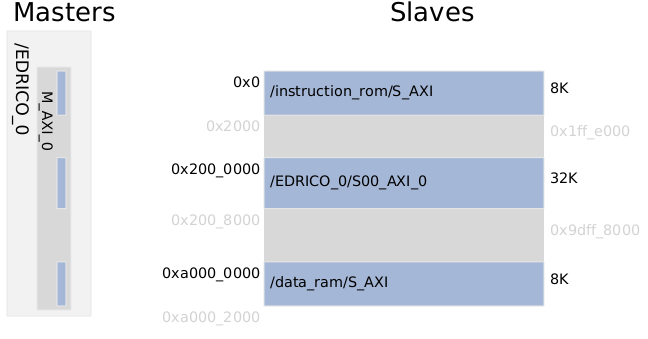
\includegraphics[width=\textwidth]{SysVer_memoryMap.png}
	\caption{memory map of the system verification test bench}
	\label{fig:SysVerMM}
\end{figure}

The instruction \ac{ROM} is defined to start at address 0x00000000 it has a size of 8KB. This is sufficient, since the test cases contain a fairly small amount of code to be executed. The same applies to the 8KB data memory at the base address of 0xA0000000.\\
In between data and instruction memory, a 32KB address space is reserved for the memory mapped \ac{CSR}.\\
\\
The test code is written in assembly, it is designed to test every RV32I instruction that is implemented. Therefore in this first test, no Zicsr instructions are tested. Hence only the \ac{GPR} and \ac{PC} contents need to be verified after execution. The \ac{IR} does not need verification, since any error in it will cause the machine to work in an undefined state, which would modify contents of the other registers to be unequal to the expected outcome.\\
Table \ref{SysVer_results} compares expected and actual register values:

\begin{table}[H]
	\setlength\arrayrulewidth{2pt}
	\centering
	\begin{tabular}{|c|c|c|c|c|c|}
		\hline
		Register & Expected  & Actual & Register & Expected & Actual \\
		\hline
		PC & 0x000000C0 & 0x00000000 & x16 & 0x0A000000 & 0x0A000000 \\
		\hline
		x1 & 0xA0000000 & 0xA0000000 & x17 & 0x00010000 & 0x00010000 \\
		\hline
		x2 & 0xC0BAD000 & 0xC0BAD000 & x18 & 0x00000000 & 0x00000000 \\
		\hline
		x3 & 0x12345000 & 0x12345000 & x19 & 0x00000001 & 0x00000001 \\
		\hline
		x4 & 0x00001000 & 0x00001000 & x20 & 0xC0BAC000 & 0xC0BAC000 \\
		\hline
		x5 & 0x000000AB & 0x000000AB & x21 & 0xC0BAD000 & 0xC0BAD000 \\
		\hline
		x6 & 0x12345014 & 0x12345014 & x22 & 0x00000000 & 0x00000000 \\
		\hline
		x7 & 0x0000C0BA & 0x0000D000 & x23 & 0x12344000 & 0x12344000 \\
		\hline
		x8 & 0x000000C0 & 0x00000000 & x24 & 0xD2EF2000 & 0xD2EF2000 \\
		\hline
		x9 & 0x12345000 & 0x13450000 & x25 & 0xF4000000 & 0xF4000000 \\
		\hline
		x10 & 0xFFFFC0BA & 0xFFFFD000 & x26 & 0x28000000 & 0x28000000 \\
		\hline
		x11 & 0xFFFFFFC0 & 0x00000000 & x27 & 0x00010000 & 0x00010000 \\
		\hline
		x12 & 0x00000000 & 0x00000000 & x28 & 0x00000000 & 0x00000000 \\
		\hline
		x13 & 0x123451EA & 0x123451EA & x29 & 0x00000001 & 0x00000001 \\
		\hline
		x14 & 0x00000004 & 0x00000004 & x30 & 0xA0000100 & 0xA0000100 \\
		\hline
		x15 & 0xFA000000 & 0xFA000000 & x31 & 0x000000B8 & 0x000000B8 \\
		\hline
	\end{tabular}
	\label{SysVer_results}
	\caption{System Verification results and expected values}
\end{table}

The test code is made up of 48 instructions, therefore the PC is expected to be:
$$PC=48*4=192=0xC0$$
after execution. When taking a look at table \ref{SysVer_results} one sees a difference between the expected and actual result for the PC. This problem is caused by the last instruction that is executed. It is a jump back to the start of the address, hence 0x00000000. After investigating the assembly code, the cause for this behavior is found. The last instruction is a \ac{JALR} instruction.

\begin{lstlisting}[caption=Snippet 1 from the executed test code]
	JAL x31, 8 #jump 8 byte
	NOP
	JALR x0, x0, 0 #jump to start
\end{lstlisting}

Therefor the \ac{PC} is set to 0x00000000. Using the simulators waveform viewer, it can be verified that the \ac{PC} prior to this instruction was set to 0x000000BC. This confirms the correct behavior of the program counter register during execution.\\
Comparing the remaining results in the table shows another error at registers x7,x8, x10 and x11. The instructions responsible for these registers are shown below:

\begin{lstlisting}[caption=Snippet 2 from the executed test code]
	SW x2, 0(x1)
	SW x3, 4(x1)
	SW x4, 8(x1)
	ADDI x5, x0, 0xAB
	SB x5, 13(x1)
	SH x2, 14(x1)
	
	LB x11, 3(x1) #expect 0xFFFFFFC0
	LH x10, 2(x1) #expect 0xFFFFC0BA
	LW x9, 4(x1) #expect 0x12345000
	LBU x8, 3(x1) #expect 0x000000C0
	LHU x7, 2(x1) #expect 0x0000C0BA
\end{lstlisting}

This code snippet shows how the memory at base address x1 is modified by multiple store word, half-word and byte instructions.
In the second part of the code x11 to x7 are modified by load instructions. It is interesting to note, that only x9 contains the expected results, and that the instruction modifying x9 is a load word instruction. To see if the error is caused by the load instructions or if the store instructions are wrong, the memory is checked. Figure \ref{fig:SysVerWV} shows the memory in the simulation wave form view:

\begin{figure}[H]
	\centering
	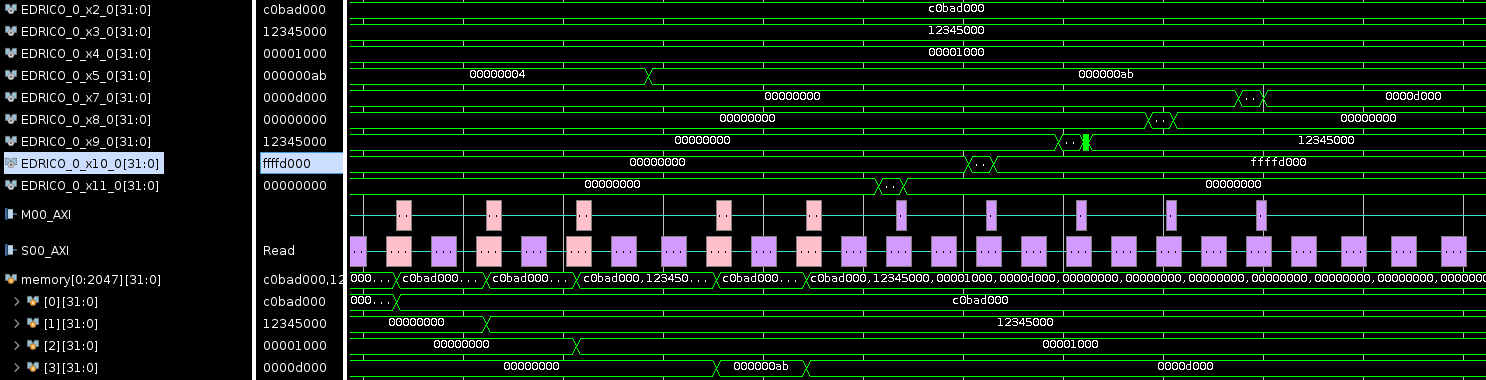
\includegraphics[width=\textwidth]{sim_EDRICO_AV_3.png}
	\caption{wave from view of the memory, AXI4-Lite transfer, x2-x5 and x7-x11 during System Verification}
	\label{fig:SysVerWV}
\end{figure}

The write transfers are displayed in the light pink-orang-ish colour whereas reads are marked in purple. As verified by comparing the memory contents with the registers x2-x4, all three store word operations are executed correctly. The store byte operation to the 0xA000000D should load 0x0000AB00 into the third memory array, followed by a store half-word to 0xA000000E which should modify the memory contents to be 0xD000AB000. However, the fourth memory element is set to 0x000000AB instead of 0x0000AB00. This is then again overwritten to be 0x0000D000. When taking a closer look at the AXI transfer everything seems fine, the right write addresses are specified and the write strobe signal (which indicates what bytes of the transfer are valid) is correct.\\
This leads to the conclusion that the mismatch in expected and actual data is not caused by the core itself. Much rather the used memory is not properly byte but word addressable. Future tests must verify this.\\
\\
One important measured value to compare processor performances is the \ac{CPI}, hence the amount of clock cycles are needed to execute an instruction. As described earlier, the \ac{CPI} is calculated using the values of the \textit{mcycle} and \textit{minstret} registers:

$$CPI = \frac{mcycleH>>32 + mcycle}{minstretH>>32 + minstret} = \frac{0x207}{0x2b} = 12.07$$

Hence in average every instruction takes 12.07 clock cycles to execute. Of course this value is highly dependent on the ratio of load/store instructions to other operations. An instruction accessing memory takes 18 cycles, whereas normal operations take 10 clock cycles. Therefore improving memory access time will decrease the CPI. Of course this assumption is very vague since, according to Amdahl's law, the improvement will not be linear \cite{patterson:2017}.
